\section{The \protein{Mad1}-\protein{Mad2} heterotetramer may adopt a fold-back conformation both \Latin{in vivo} and \Latin{in vitro}}

For the ``knitting'' model to work, the cell need to position the site of \protein{Mad2}'s conformational switch and \protein{Cdc20}'s MIM close enough. According to the crystal structure, the axial length from the MIM to the start of the loop region is about 5--\SI{6}{nm} while the axial length from the end of the loop region to the anchoring point of \protein{Cdc20} is about \SI{7}{nm} \cite{TemplateModel, Ji2017eLife, BUB1-CDC20-MAD1, Structure1GO4, Structure4DZO}. In contrast, if we model the disordered N-termnius of \protein{Cdc20} as a simple 3-D random walk, we can estimate the root-mean-square distance from \protein{Cdc20}'s BOX1 to its MIM (about 90 residues) to be less than \SI{4}{nm}. Due to steric hinderance and restrictions imposed by the Ramachandran plot, such a simple 3-D random walk model is far from realistic. However, even if we apply a more sophisticated worm-like chain model with a persistence length of 3--\SI{4}{\angstrom} \cite{RandomWalk3D-WormLikeChain}, the root-mean-square distance from \protein{Cdc20}'s BOX1 to its MIM is still only about \SI{5}{nm}. These estimations suggest that additional mechanisms may be at work to position the site of \protein{Mad2}'s conformational switch and \protein{Cdc20}'s MIM closely to facilitate the heterodimerization between \protein{Mad2} and \protein{Cdc20}.

One possibility has been suggested in \cite{BUB1-CDC20-MAD1, Tripartite} that the cooperative binding of \protein{Cdc20} to \protein{Mad1}'s RWD domain and \protein{Bub1} helps to unravel the N-terminus of \protein{Cdc20}. Indeed, if the disordered region from \protein{Cdc20}'s BOX1 to its MIM is fully stretched, it will be more than enough for the MIM of the \protein{Cdc20} anchored to \protein{Mad1}'s RWD domain to engage the site of \protein{Mad2}'s conformational switch. However, there are conflicting claims over whether and where \protein{Bub1} directly binds to \protein{Mad1} \cite{Ji2017eLife, BUB1-CDC20-MAD1, BUB1CD1-MAD1CStructure}. If \protein{Bub1}'s conserved domain 1 (CD1, which is also named conserved motif 1 or CM1) directly interacts with \protein{Mad1}'s consensus RLK motif located in \protein{Mad1}'s C-terminal coiled coil \cite{Ji2017eLife, BUB1CD1-MAD1CStructure} (illustrated in \myref{KnittingModel} as the contact between \protein{Bub1} and the C-terminal coiled coil of \protein{Mad1}), the cooperative binding of \protein{Cdc20} to \protein{Bub1} and \protein{Mad1} may not unravel \protein{Cdc20}'s N-terminus because the segment of \protein{Bub1} from CD1 to ABBA-consensus KEN motifs (which bind to \protein{Cdc20} \cite{BUB1-CDC20-MAD1, CDC20-KEN, ABBA}) is also largely disordered (predicted by AlphaFold2 with low confidence; data not shown).

Another possibility has been suggested in \cite{Structure1GO4, SpMad1} that \protein{Mad1} may position the site of \protein{Mad2}'s conformational switch and \protein{Cdc20}'s MIM closely by assuming a fold-back conformation. As mentioned in the previous section, the secondary structure of \protein{Mad1}'s C-terminal loop region is conserved, whose flexibility may enable such fold-back conformation according to the prediction by the ColabFold advanced algorithm (see \myref{MAD1_ColabFoldPrediction}, which is close to the scenario envisioned by \cite{SpMad1}). If we truncate residues 582--600 of human \protein{Mad1}, which removes the flexible loop and fuses the coiled coils upstream and downstream of the loop region (while preserving the original heptad repeat position designation as assigned by Lupas' method \cite{LupasCOILS} as well as DeepCoil2 \cite{DeepCoil}; data not shown), the resulting loop-deleted \protein{Mad1} (henceforth referred to as \protein{Mad1}\textDelta{}L) homodimer can only assume an extended conformation (see \myref{MAD1DeltaL_ColabFoldPrediction}).

\begin{figure}
    \centering
    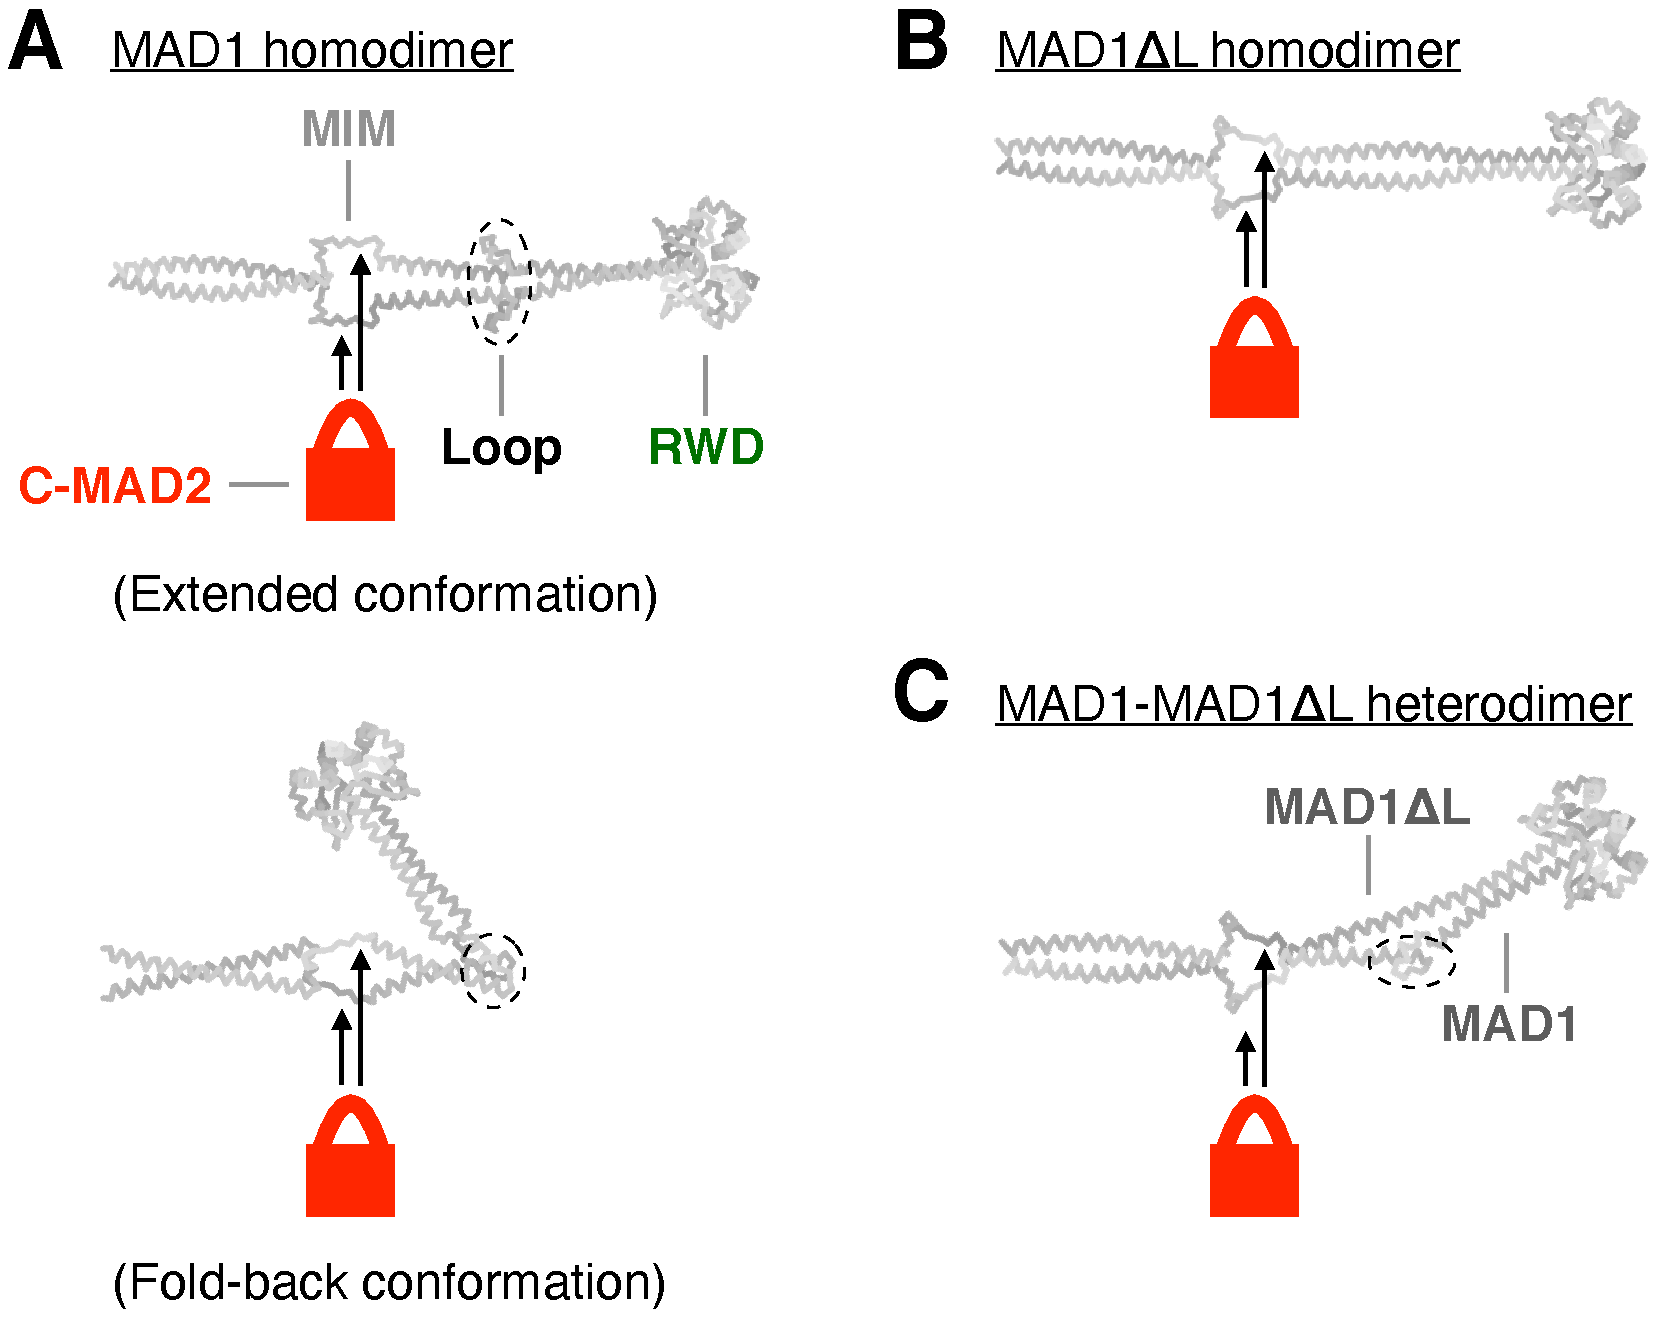
\includegraphics[width=0.77\textwidth]{chapters/figures/ColabFoldPrediction.pdf}
    \phantomsubfiglabel{MAD1_ColabFoldPrediction} % subfigure A
    \phantomsubfiglabel{MAD1DeltaL_ColabFoldPrediction} % subfigure B
    \phantomsubfiglabel{MAD1-MAD1DeltaL_ColabFoldPrediction} % subfigure C
    \caption{\textbf{Representative structures of the C-terminus of the \protein{Mad1} homodimer, the \protein{Mad1}\textDelta{}L homodimer, and the \protein{Mad1}-\protein{Mad1}\textDelta{}L heterodimer were predicted by ColabFold.}}
    \noindent\justifying Representative models (out of five models in total) of the C-terminus of the \protein{Mad1} homodimer (A), the \protein{Mad1}\textDelta{}L homodimer (B), and the \protein{Mad1}-\protein{Mad1}\textDelta{}L heterodimer (C) were predicted by ColabFold using the default parameter settings of ColabFold advanced algorithm. The loop region of wildtype \protein{Mad1} is circled out in (A) and (C). The MIM of \protein{Mad1} where C-\protein{Mad2} binds and the RWD domain at the C-terminal end of \protein{Mad1} where the N-terminal BOX1 of \protein{Cdc20} is anchored are also indicated. The C-terminus of the \protein{Mad1} homodimer may assume a fold-back conformation [see the bottom panel of (A)]. In the structure of the \protein{Mad1}-\protein{Mad1}\textDelta{}L heterodimer, the loop region of the wildtype copy introduces a bulge but the overall conformation is extended. 
    \label{ColabFoldPrediction}
\end{figure}

To confirm such fold-back of \protein{Mad1}, we first noted that about 37\% of purified full-length \protein{Mad1}-\protein{Mad2} heterotetramers do not show distinguishable \protein{Mad1}-MIM-\protein{Mad2} and \protein{Mad1}-RWD domain densities as visualized by electron microscopy using metal shadowing \cite{BUB1-CDC20-MAD1}. This may be explained by that this population of \protein{Mad1}-\protein{Mad2} heterotetramers assumes a fold-back conformation. To further support that the \protein{Mad1} may assume a fold-back conformation \Latin{in vivo}, we resorted to the distance-sensitive FRET measurement. We fused the donor fluorophore mNeonGreen to the C-terminal end of \protein{Mad1} (see \myref{TaggingSACProteins}) and inserted the acceptor fluorophore mScarlet-I into the \textbeta{}5-\textalpha{}C loop of \protein{Mad2} \cite{mSI, beta5-alphaCLoop}. If \protein{Mad1} always assumes an extended conformation, the distance between the donor and acceptor will be larger than \SI{10}{nm}, which allows no or minimal FRET between the donor and the acceptor. However, if \protein{Mad1} may assume a fold-back conformation, the distance between the donor and acceptor may be reduced to allow for FRET between the donor and the acceptor.

We first confirmed the expression of \protein{Mad2}$\wedge$mScarlet-I in the \gene{Mad2}$\wedge$mScarlet-I genome-edited HeLa-A12 cell line and that \protein{Mad2}$\wedge$mScarlet-I could support the SAC signaling when cells were treated with \SI{50}{nM} nocodazole. Using fluorescence lifetime imaging microscopy (FLIM), we observed FRET at an efficiency of about 3--4\% between \protein{Mad1}-mNG and \protein{Mad2}$\wedge$mScarlet-I at the interphase/prophase NPC in the heterozygous \gene{Mad1}-mNG, \gene{Mad2}$\wedge$mScarlet-I genome-edited HeLa-A12 cell line. We chose to measure FRET at the interphase/prophase NPC to facilitate data collection by the line-scanning confocal microscope and to avoid the potential inter-molecular FRET between the donor mNeonGreen on one \protein{Mad1}-\protein{Mad2} heterotetramer and the acceptor mScarlet-I at another nearby heterotetramer at the corona of a signaling kinetochore. This FRET still existed even when \gene{Cdc20} was knocked down by RNAi, which indicates that this phenomenon does not depend on \protein{Mad1}'s catalytic role but is rather intrinsic to the structural characteristics of the \protein{Mad1}-\protein{Mad2} heterotetramer. Although we still cannot rule out the possibility of inter-molecular FRET, we at least confirmed the existence of the anticipated FRET that may result from the fold-back of \protein{Mad1} \Latin{in vivo}.
%  

% Functionality of MAD2^mSI figure

\section{\protein{Mad1}'s loop region is important to the SAC signaling activity \Latin{in vivo}}
\label{LoopDeletionSection}

We next sought to determine whether the loop region that likely enabled the fold-back conformation of \protein{Mad1} is important to the SAC signaling activity \Latin{in vivo}. We integrated the expression cassette of either \protein{Mad1}-mNG or \protein{Mad1}\textDelta{}L-mNG into the genome of HeLa-A12 cells using Cre-\bacterialgene{lox} RMCE (see \myref{Cre-lox}). We then knocked down endogenous \protein{Mad1} in these stably-transfected cells using siRNAs that target the 3'-UTR of \gene{Mad1} \cite{siMAD1-3UTR} (henceforth collectively referred to as si\gene{Mad1}) and induced the expression of \protein{Mad1}(WT/\textDelta{}L)-mNG (si\gene{Mad1}-resistant due to their lack of the endogenous 3'-UTR) by doxycycline. Our genome-edited \gene{Mad1}-mNG HeLa-A12 cell line served as a reference of the endogenous level of \protein{Mad1} in our live-cell fluorescence imaging.

We found out that knocking down \gene{Mad1} by transfecting the cells with si\gene{Mad1} for two days crippled the SAC signaling activity. However, cells with less than 10\% of the physiological level of \protein{Mad1} on average (estimated from the immunoblot in \myref{MAD1Rescue_WB}) still arrested in mitosis for a considerable amount of time when treated with \SI{100}{nM} nocodazole (only about two hours less than the control group with a physiological level of \protein{Mad1}), indicating that even a small pool of \protein{Mad1} could sustain a considerable level of SAC signaling activity.

% figure
% \myref{MAD1Rescue_WB}
% add t-test between knockdown and knockdown + ∆L

Wildtype \protein{Mad1}-mNG fully rescued cells treated with si\gene{Mad1}. Surprisingly, \protein{Mad1}\textDelta{}L had impaired support for the SAC in a dominant-negative manner: cells treated with si\gene{Mad1} and were rescued by a physiological level of \protein{Mad1}\textDelta{}L arrested in mitosis for a significantly shorter duration than cells which were not rescued. One possible explanation was that \protein{Mad1}\textDelta{}L-mNG dimerized with the remaining endogenous \protein{Mad1} and restricted its structural flexibility. Structural prediction of the heterodimer between wildtype \protein{Mad1} and \protein{Mad1}\textDelta{}L showed that the loop region of the wildtype \protein{Mad1} introduced a bulge but not enabling the fold-back conformation due to stiffness of the fused \textalpha{}-helix of \protein{Mad1}\textDelta{}L (see \myref{MAD1-MAD1DeltaL_ColabFoldPrediction}). To experimentally confirm this hypothesis, we pulled down doxycycline-induced \protein{Mad1}(wildtype/\textDelta{}L)-mNG from the lysates of HeLa-A12 cells wherein the endogenous \protein{Mad1} was not knocked down. We found that endogenous \protein{Mad1} was also pulled down by both \protein{Mad1}-mNG and \protein{Mad1}\textDelta{}L-mNG, but not by mNeonGreen alone. This proves that the ectopic recombinant \protein{Mad1}\textDelta{}L-mNG can indeed heterodimerize with endogenous \protein{Mad1}.

To confirm that the defect in the SAC signaling activity observed in cells rescued by \protein{Mad1}\textDelta{}L was not due to potential defect in its interaction with \protein{Mad2} or any unexpected effect on the expression of certain SAC proteins, we quantified the localization of \protein{Mad2} at signaling kinetochores by fluorescence imaging and quantified the expression level of other SAC proteins by immunoblotting. Genome-edited \gene{Mad2}$\wedge$mScarlet-I HeLa-A12 cells treated with si\gene{Mad1} and rescued by \protein{Mad1}(wildtype/\textDelta{}L)-mNG showed that no difference in the localization of either \protein{Mad1} or \protein{Mad2} at signaling kinetochores. The cellular abundance of some other SAC proteins like \protein{BubR1}, \protein{Cdc20}, and \protein{Bub3} was also not affected by the rescue experiment (see \myref{MAD1Rescue_WB}).

\Latin{In vitro} reconstitution data (not shown here) from our collaborator also suggested that truncating the loop region of \protein{Mad1} reduced the rate of the formation of \protein{Cdc20}-\protein{Mad2}. Although the results of our knockdown-rescue experiment may have been influenced by the incomplete knockdown of the endogenous \protein{Mad1}, all of these experiments together proved that the loop region of \protein{Mad1} is critical to the SAC signaling activity in its own right.